%!TEX root = ./report.tex

\section{Control and Observation}
Below one can find the implementation and results of the close-loop state feedback LQR controller.
Additionally, the results and implementation using a state observer are shown.

\subsection{LQR Design and Implementation}
Given the cost matrices and the linear system model, the LQR gain is computed using the MATLAB function \texttt{dlqr} or alternatively using the Ricatti recursive formula.
In order to observe the convergence of the Ricatti iteration, the singular values of the matrix $\bb{S}_n$ are observed.
For $\bb{Q}_1 = \diag (0, 1, 1, 1, 1)$ and $\bb{Q}_2 = \diag (1, 1)$ the convergence shows a profile as in Figure~\ref{fig:ricatti_svds}.
For other settings of the cost matrices the convergence looks slightly different.
Therefore, to have some margin for guaranteed convergence upon variance of the cost function, the iteration number is set to $n_{iterations} = 2500$.

\begin{figure}[h]
	\centering
	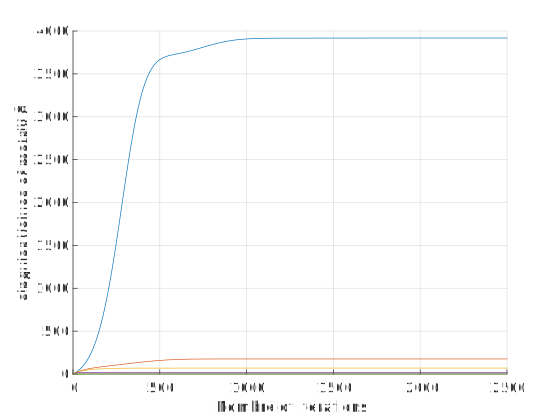
\includegraphics[width=.5\textwidth]{figures/svds.pdf}
	\caption{Evolution of the singular values of $\bb{S}_n$ during the Ricatti iteration.}
	\label{fig:ricatti_svds}
\end{figure}

Given the LQR gain matrix, it is used as state feedback gain in a closed-loop fashion.
Figure~\ref{fig:lqr_closed} shows the implementation in \textsc{Simulink}.

\begin{figure}[h!]
	\centering
	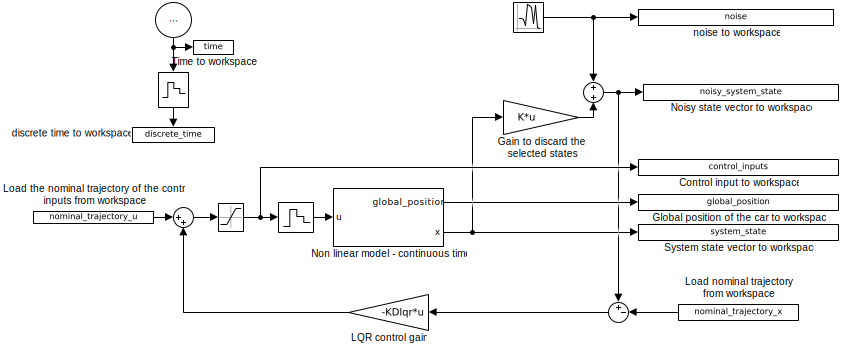
\includegraphics[width=\textwidth]{figures/lqr_closed_loop.pdf}
	\caption{\textsc{Simulink} implementation of the LQR state feedback controller. The LQR state feedback is added to the nominal trajectory for the control input and the sum signal is fed to the system model via a saturation and zero-order hold block. Then, the system output is distorted by noise and certain states are neglected. After subtracting the nominal state trajectory, the state signal is fed to the controller.}
	\label{fig:lqr_closed}
\end{figure}

\subsection{LQR Assessment with Ideal Information}

The closed-loop system including the controller is simulated using the second reference path and the results are presented in Figure~\ref{fig:lqr_closed_results}.
The simulation is run for different settings of the cost function, while the first weight for the state cost function is always zero.
On the top left (a) the identically weighted cost function is used and in (b) the weights for the angular values are increased by a factor of $10$.
A higher cost for angle errors leads to higher lateral deviations (state $2$) and lower control input for the steering angle at the same time.
In contrast to that, the lateral deviation is nearly ignored in (c) and only the heading error is considered for control.
In order to obtain a good performance the weight for the lateral deviation is increased and the behavior as in (d) is observed. 
At $t \approx 60s$ the vehicle slightly oscillates around the reference trajectory in the sharp curve, which is undesirable.
To get rid of the oscillation, the cost for steering is decreased, which results in an unstable behavior.
In particular, the system starts to oscillate uncontrollably at the critical sharp curve at $t \approx 60s$ (e).
Finally, by decreasing the weight for the lateral deviation again, a nice performance without oscillations for the settings shown in Figure~\ref{fig:lqr_closed_results} (f) is achieved.

\begin{figure}[h!]
	\centering
	\begin{subfigure}{0.32\textwidth}
		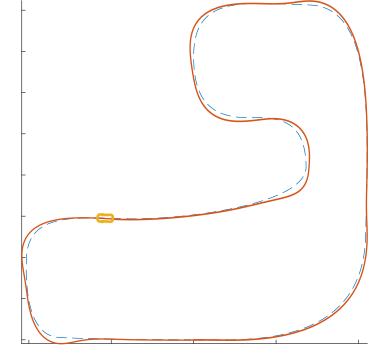
\includegraphics[width=.9\textwidth]{figures/clean_1_path.pdf}
		\includegraphics[width=\textwidth]{figures/clean_1_input.png}
		\subcaption{$\bb{Q}_1=\diag(0, 1, 1, 1, 1)$,\\$\bb{Q}_2=\diag(1, 1)$}
	\end{subfigure}
	\begin{subfigure}{0.32\textwidth}
		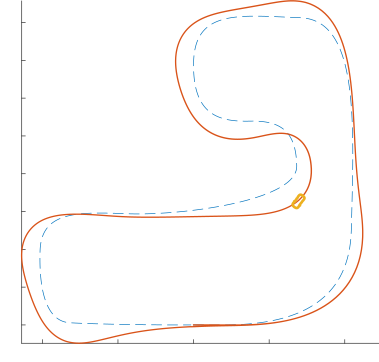
\includegraphics[width=.9\textwidth]{figures/clean_2_path.pdf}
		\includegraphics[width=\textwidth]{figures/clean_2_input.png}
		\subcaption{$\bb{Q}_1=\diag(0, 1, 100, 1, 100)$,\\$\bb{Q}_2=\diag(1, 100)$}
	\end{subfigure}
	\begin{subfigure}{0.32\textwidth}
		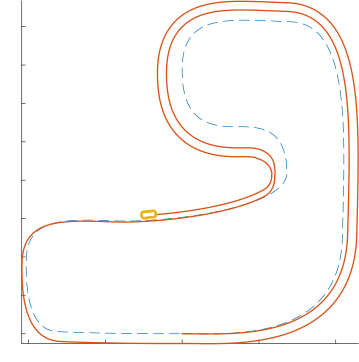
\includegraphics[width=0.9\textwidth]{figures/clean_6_path.pdf}
		\includegraphics[width=\textwidth]{figures/clean_6_input.png}
		\subcaption{$\bb{Q}_1=\diag(0, 10^{-4}, 500, 1, 1)$,\\$\bb{Q}_2=\diag(1, 0.5)$}
	\end{subfigure}
	\begin{subfigure}{0.32\textwidth}
		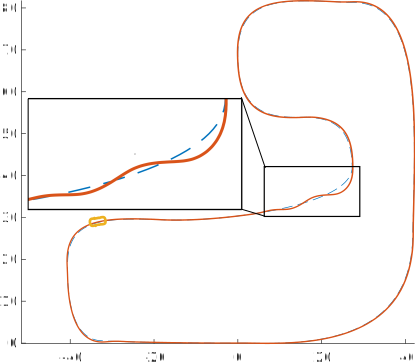
\includegraphics[width=0.9\textwidth]{figures/clean_3_path.pdf}
		\includegraphics[width=\textwidth]{figures/clean_3_input.png}
		\subcaption{$\bb{Q}_1=\diag(0, 100, 1, 1, 1)$,\\$\bb{Q}_2=\diag(1, 1)$}
	\end{subfigure}
	\begin{subfigure}{0.32\textwidth}
		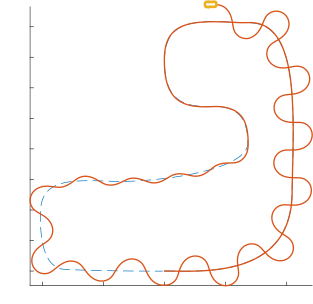
\includegraphics[width=0.9\textwidth]{figures/clean_5_path.pdf}
		\includegraphics[width=\textwidth]{figures/clean_5_input.png}
		\subcaption{$\bb{Q}_1=\diag(0, 100, 1, 1, 1)$,\\$\bb{Q}_2=\diag(1, 0.5)$}
	\end{subfigure}
	\begin{subfigure}{0.32\textwidth}
		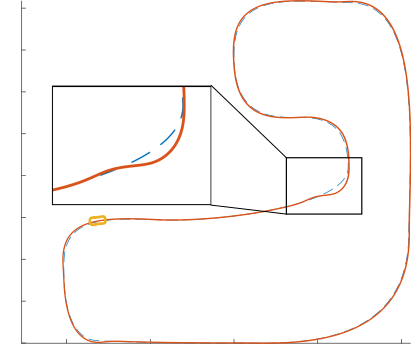
\includegraphics[width=0.9\textwidth]{figures/clean_4_path.pdf}
		\includegraphics[width=\textwidth]{figures/clean_4_input.png}
		\subcaption{$\bb{Q}_1=\diag(0, 5, 1, 1, 1)$,\\$\bb{Q}_2=\diag(1, 0.5)$}
	\end{subfigure}
	\caption{Resulting vehicle path (red line) as response to the reference trajectory (blue dashed line) using the closed-loop state feedback LQR controller. The experiment is run for different setting of the cost function.}
	\label{fig:lqr_closed_results}
\end{figure}

\subsection{LQR Assessment with Imperfect Information}
Below, the performance of the closed-loop system with only imperfect information is evaluated.
From now on, the weights for the cost functions are fixed to the good performing values from Figure~\ref{fig:lqr_closed_results} (f) being $\bb{Q}_1=\diag(0, 5, 1, 1, 1)$ and $\bb{Q}_2=\diag(1, 0.5)$.

\paragraph{Adding Noise to the Fully Observable State:} A zero-mean Gaussian noise signal with standard deviations $\left[1, 1, 0.1745, 2, 0\right]$ is added to the state output as shown in Figure~\ref{fig:lqr_closed}. 
The noise level is comparably high, but the vehicle still can follow the path, with some inaccuracies though (a).
As the control signal is a linear mapping of the observed state vector, also the control signal is highly noisy as there is no filtering at all.
The controller is purely proportional in the measured states and has no filtering effects.
Consider, for instance, the reference angle for the steering angle $u_2$ in (b). 
The control input is noisy and saturates nearly everywhere.
However, the actuator dynamics (eq.~\ref{eq:ss5}) of the system have low pass behavior and filter out the noise from the control input.
In the diagram showing the evolution of the states (c) it is observable that the actual steering angle shows the filtered version of the control input with nearly no noise (state 5).

As we have zero-mean noise and the actuators have low-pass behavior (eq. \ref{eq:ss4} and \ref{eq:ss5}) the closed-loop system still behaves properly and the accuracy is reasonable even with this comparatively high level of noise.

\begin{figure}[h]
	\centering
	\begin{minipage}{0.4\textwidth}
		\begin{subfigure}{\textwidth}
				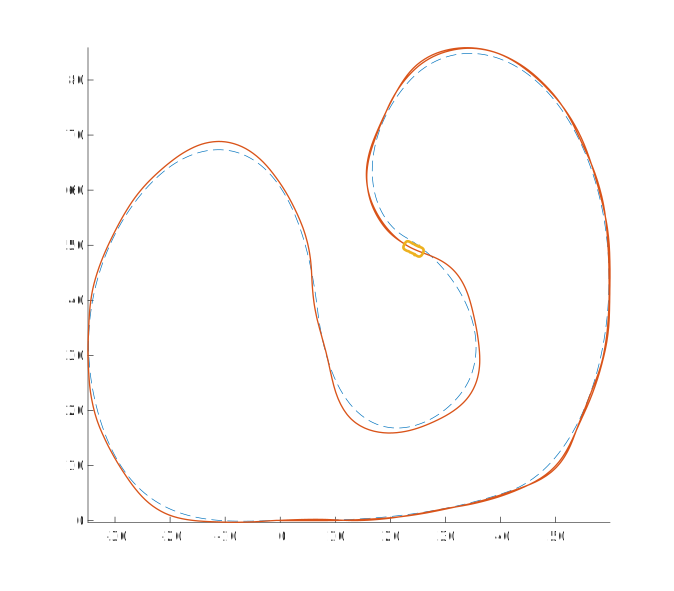
\includegraphics[width=\textwidth]{figures/noisy_1_path.pdf}
				\subcaption{Path}	
		\end{subfigure}
		\begin{subfigure}{\textwidth}
				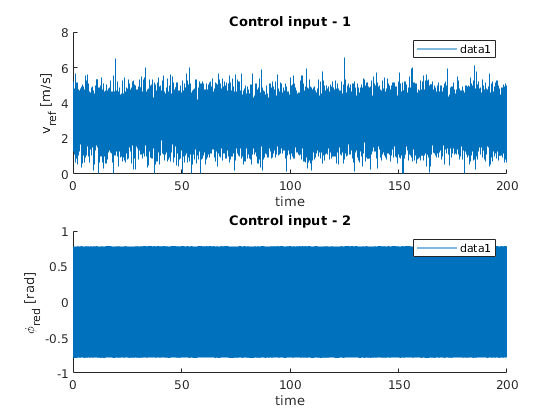
\includegraphics[width=\textwidth]{figures/noisy_1_inputs.pdf}
				\subcaption{Input}
		\end{subfigure}
	\end{minipage}
	\begin{subfigure}{.59\textwidth}
		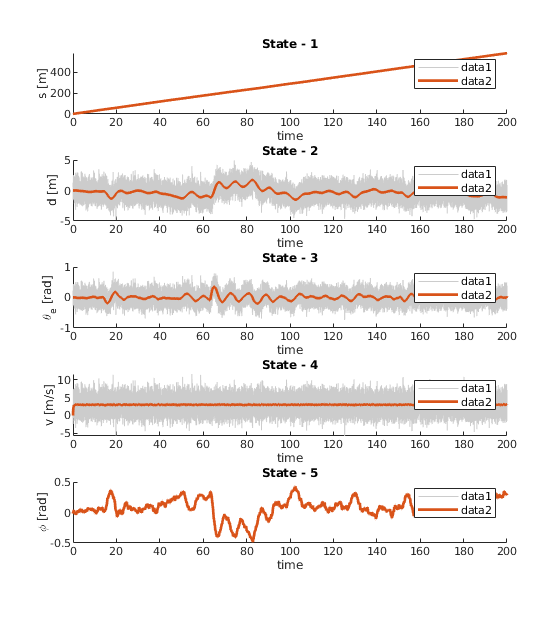
\includegraphics[width=\textwidth]{figures/noisy_1_states.pdf}
		\subcaption{States}	
	\end{subfigure}
	\caption{Performance of the LQR state feedback controller, when the state signal is distorted by noise. As the control signal is a linear mapping of the observed state vector without integrators or filters, the control signal is noisy as well. However, the system actuators have low-pass behavior and filter out the noise and the system still behaves properly and follow the path with small inaccuracies. Note that zero-mean Gaussian noise is used.}
	\label{fig:noisy_states}
\end{figure}

\paragraph{Neglecting a State: } In addition, one of the states is neglected and not fed to the controller.
In particular, we neglect the third state expressing the heading error $\theta_e$, i.e. the controller has no information about the heading error of the vehicle.
Note, that the noise is still activated with the same settings as before.
The resulting system behavior is shown in Figure~\ref{fig:partially_states}.
In this setting, the controller always thinks the heading error is zero and the vehicle does not properly track the path.
After some time the control input for the reference steering angle is saturated all the time and the vehicle keeps moving in small circles.
Even though there are some small peaks with positive sign, these are filtered out by the low-pass behavior of the steering wheel actuator and the steering wheel stays approximately at $-\frac{\pi}{2}$.
For the selected cost function, the LQR state-feedback gain matrix is
\begin{equation}
	\bb{K}_{D_{LQR}} = \begin{bmatrix}
	0.0000 &  -0.0000  & -0.0000  &  0.4069 &  -0.0000\\
    0.0000  &  3.1360 &  10.5130 &  -0.0000  &  3.3271	
	\end{bmatrix}\, .
\end{equation}
Accordingly, the reference steering angle is affected by the lateral deviation $x_2$, the heading error $x_3$ and the actual steering angle $x_5$. 
Here, the measured heading error is always zero and the control input $u_2$ is a linear combination of the lateral deviation and the steering wheel angle.
As the lateral deviation becomes large and the actual steering angle can not go beyond $-\frac{\pi}{2}$ and $\frac{\pi}{2}$ the feedback value is nearly always positive as the lateral deviation is large.
The inverse of that positive signal is fed back to the system, saturates the saturation block and results in a maximally deflected steering wheel.
The system becomes unstable and the vehicle traces out small circles forever.

\begin{figure}[h]
	\begin{minipage}{0.4\textwidth}
		\begin{subfigure}{\textwidth}
				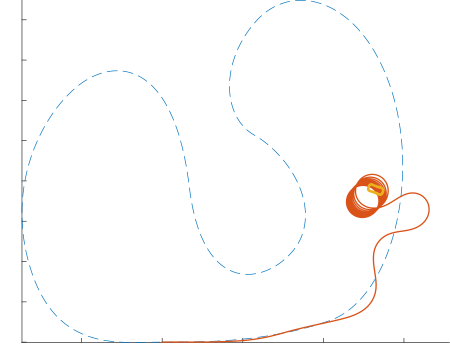
\includegraphics[width=\textwidth]{figures/partially_1_path.pdf}
				\subcaption{Path}	
		\end{subfigure}
		\begin{subfigure}{\textwidth}
				\includegraphics[width=\textwidth]{figures/partially_1_inputs.png}
				\subcaption{Input}
		\end{subfigure}
	\end{minipage}
	\begin{subfigure}{.59\textwidth}
		\includegraphics[width=\textwidth]{figures/partially_1_states.png}
		\subcaption{States}	
	\end{subfigure}
	\caption{Performance of the LQR state feedback controller neglecting the heading error state for feedback.}
	\label{fig:partially_states}
\end{figure}

\subsection{State Observer}
Figure~\ref{fig:lqr_and_observer} shows the implementation of the closed-loop system including the LQR state feedback controller, the vehicle model and the observer.
The observer operates on nominal states and requires the nominal control input as well.
It infers the non-measurable heading error state ($x_3$) given the remaining available states.
Note, that the observer outputs the estimated nominal states, not the global ones.
As the saturation acts on the global control input signal, the nominal control input must first be added and later subtracted in order to obtain a correct control input feedback signal for the observer.

\begin{figure}[h]
	\centering
	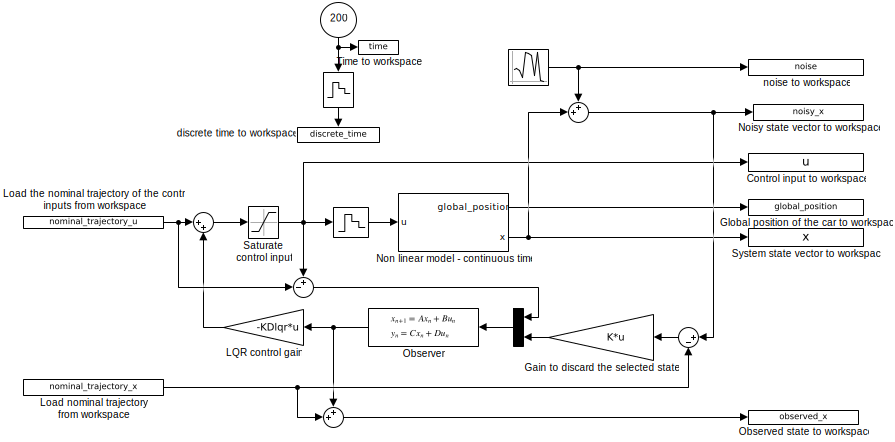
\includegraphics[width=\textwidth]{figures/lqr_observer.pdf}
	\caption{\textsc{Simulink} implementation of the LQR feedback controller combined with a state observer to infer neglected states.}
	\label{fig:lqr_and_observer}
\end{figure}

Further, the observer poles $\lambda_{obs,i}$ are set to some percentage of the poles of the linearized system $\lambda_{sys,i}$.
The smaller the observer poles the faster the convergence of the estimated states, but also the sensitivity to noise grows and the observed states might just follow the noise signal.
On the other hand, larger poles (close to $100\%$ of the system poles) have more filtering effect of noise, but require longer convergence times.
Figure~\ref{fig:observer_result_paths} shows resulting paths of the vehicle using the observer and different settings for the poles.
Additionally, Figure~\ref{fig:observer_result_states} shows the measured, estimated and true states for two of these settings.
For a percentage of $100\%$ the noise is filtered out for the non-measured states while at $95\%$ the noise is already followed.

\begin{figure}[h]
	\begin{subfigure}{0.24\textwidth}
		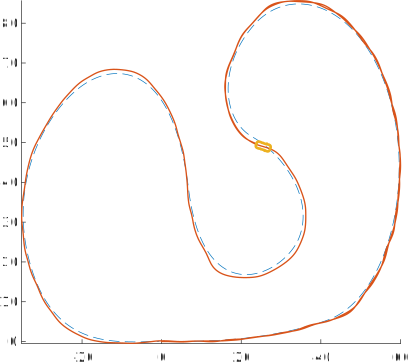
\includegraphics[height=0.8\textwidth]{figures/observer_100_path.pdf}
		\subcaption{$\lambda_{obs,i} = 100\% \cdot \lambda_{sys,i}$}
	\end{subfigure}
	\begin{subfigure}{0.24\textwidth}
		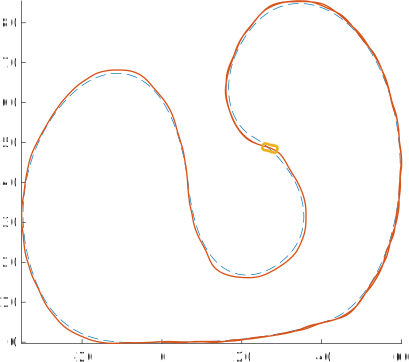
\includegraphics[height=0.8\textwidth]{figures/observer_99_path.pdf}
		\subcaption{$\lambda_{obs,i} = 99\% \cdot \lambda_{sys,i}$}
	\end{subfigure}
	\begin{subfigure}{0.24\textwidth}
		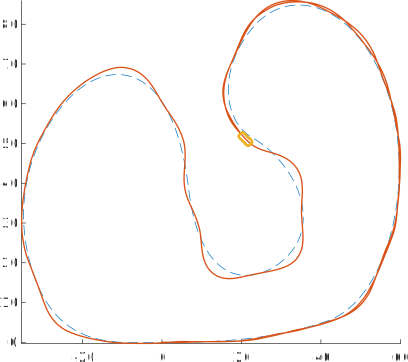
\includegraphics[height=0.8\textwidth]{figures/observer_95_path.pdf}
		\subcaption{$\lambda_{obs,i} = 95\% \cdot \lambda_{sys,i}$}
	\end{subfigure}
	\begin{subfigure}{0.24\textwidth}
		\centering
		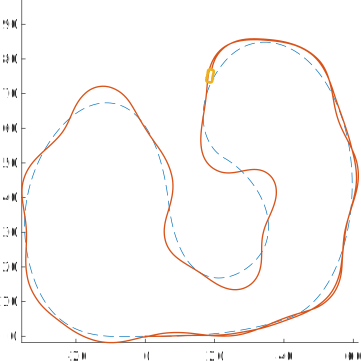
\includegraphics[height=0.8\textwidth]{figures/observer_90_path.pdf}
		\subcaption{$\lambda_{obs,i} = 90\% \cdot \lambda_{sys,i}$}
	\end{subfigure}
	\begin{subfigure}{0.24\textwidth}
		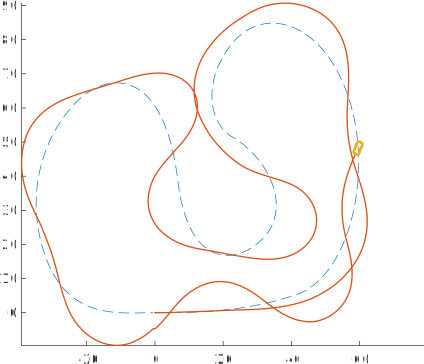
\includegraphics[height=0.8\textwidth]{figures/observer_75_path.pdf}
		\subcaption{$\lambda_{obs,i} = 75\% \cdot \lambda_{sys,i}$}
	\end{subfigure}
	\begin{subfigure}{0.24\textwidth}
		\centering
		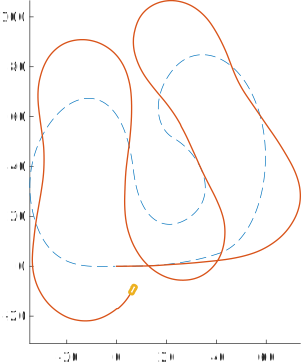
\includegraphics[height=0.8\textwidth]{figures/observer_50_path.pdf}
		\subcaption{$\lambda_{obs,i} = 50\% \cdot \lambda_{sys,i}$}
	\end{subfigure}
	\begin{subfigure}{0.24\textwidth}
		\includegraphics[width=\textwidth]{figures/observer_30_path.pdf}
		\subcaption{$\lambda_{obs,i} = 30\% \cdot \lambda_{sys,i}$}
	\end{subfigure}
	\begin{subfigure}{0.24\textwidth}
		\centering
		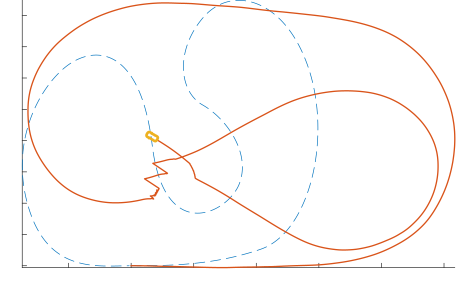
\includegraphics[width=\textwidth]{figures/observer_10_path.pdf}
		\subcaption{$\lambda_{obs,i} = 10\% \cdot \lambda_{sys,i}$}
	\end{subfigure}
	\caption{Resulting vehicle paths for different settings for the observer poles.}
	\label{fig:observer_result_paths}
\end{figure}

\begin{figure}[h]
	\begin{subfigure}{0.49\textwidth}
		\includegraphics[width=\textwidth]{figures/observer_100_states.png}
		\subcaption{$\lambda_{obs,i} = 100\% \cdot \lambda_{sys,i}$}
	\end{subfigure}	
	\begin{subfigure}{0.49\textwidth}
		\includegraphics[width=\textwidth]{figures/observer_95_states.png}
		\subcaption{$\lambda_{obs,i} = 95\% \cdot \lambda_{sys,i}$}
	\end{subfigure}	
	\caption{Observed states, measured states and true states for different settings of the observer poles. The heading error (state 3) is not measured by the observer and can be inferred. Using the system poles as observer poles, the noise is filtered out for the observed heading error. However, already at $95\%$ of the system poles, the observer follows the noise.}
	\label{fig:observer_result_states}
\end{figure}